%────────────────────────────────────────────────────────────────────────────────
%  Document AI Chatbot — Complete Project Report & Interview Preparation Guide
%────────────────────────────────────────────────────────────────────────────────
\documentclass[12pt,a4paper]{article}

% ── Packages ──────────────────────────────────────────────────────────────────
\usepackage[utf8]{inputenc}
\usepackage[T1]{fontenc}
\usepackage{lmodern}
\usepackage[margin=2.5cm]{geometry}
\usepackage{graphicx}
\usepackage{hyperref}
\usepackage{xcolor}
\usepackage{listings}
\usepackage{enumitem}
\usepackage{titlesec}
\usepackage{fancyhdr}
\usepackage{tcolorbox}
\usepackage{booktabs}
\usepackage{longtable}
\usepackage{amsmath}
\usepackage{tikz}
\usetikzlibrary{shapes.geometric, arrows.meta, positioning, fit}

% ── Colours ───────────────────────────────────────────────────────────────────
\definecolor{accentblue}{HTML}{3b6ef6}
\definecolor{codebg}{HTML}{f5f5f0}
\definecolor{codeframe}{HTML}{d0d0c8}
\definecolor{darkgreen}{HTML}{2a9d63}

% ── Hyperref setup ────────────────────────────────────────────────────────────
\hypersetup{
  colorlinks  = true,
  linkcolor   = accentblue,
  urlcolor    = accentblue,
  citecolor   = accentblue,
}

% ── Listings style ────────────────────────────────────────────────────────────
\lstset{
  backgroundcolor = \color{codebg},
  frame           = single,
  rulecolor       = \color{codeframe},
  basicstyle      = \ttfamily\small,
  keywordstyle    = \bfseries\color{accentblue},
  commentstyle    = \itshape\color{gray},
  stringstyle     = \color{darkgreen},
  breaklines      = true,
  showstringspaces= false,
  tabsize         = 4,
  numbers         = left,
  numberstyle     = \tiny\color{gray},
  numbersep       = 8pt,
}

% ── tcolorbox styles ─────────────────────────────────────────────────────────
\newtcolorbox{interviewbox}[1][]{
  colback    = blue!3,
  colframe   = accentblue,
  fonttitle  = \bfseries,
  title      = {#1},
  arc        = 3pt,
  boxrule    = 0.8pt,
  left       = 8pt,
  right      = 8pt,
}

\newtcolorbox{answerbox}{
  colback    = green!3,
  colframe   = darkgreen,
  arc        = 2pt,
  boxrule    = 0.5pt,
  left       = 8pt,
  right      = 8pt,
}

\newtcolorbox{notebox}{
  colback    = yellow!5,
  colframe   = orange!60!black,
  fonttitle  = \bfseries,
  title      = {Key Point},
  arc        = 2pt,
  boxrule    = 0.5pt,
  left       = 8pt,
  right      = 8pt,
}

% ── Header/Footer ────────────────────────────────────────────────────────────
\pagestyle{fancy}
\fancyhf{}
\fancyhead[L]{\small Document AI Chatbot — Project Report}
\fancyhead[R]{\small\thepage}
\renewcommand{\headrulewidth}{0.4pt}

% ── Section formatting ───────────────────────────────────────────────────────
\titleformat{\section}{\Large\bfseries\color{accentblue}}{\thesection}{1em}{}
\titleformat{\subsection}{\large\bfseries}{\thesubsection}{0.8em}{}
\titleformat{\subsubsection}{\normalsize\bfseries}{\thesubsubsection}{0.6em}{}

% ══════════════════════════════════════════════════════════════════════════════
\begin{document}

% ── Title Page ────────────────────────────────────────────────────────────────
\begin{titlepage}
  \centering
  \vspace*{3cm}
  {\Huge\bfseries\color{accentblue} Document AI Chatbot}\\[0.6cm]
  {\LARGE RAG-Based Study Assistant}\\[1.2cm]
  {\Large Complete Project Report \\ \& Interview Preparation Guide}\\[2cm]
  {\large\textbf{Author:} Mani}\\[0.4cm]
  {\large\textbf{Technology:} Python · FastAPI · LangChain · ChromaDB · Gemini}\\[0.4cm]
  {\large\textbf{Repository:} \href{https://github.com/mani30mk/Document-AI-Chatbot}{github.com/mani30mk/Document-AI-Chatbot}}\\[2cm]
  {\large July 2026}
  \vfill
\end{titlepage}

\tableofcontents
\newpage

%══════════════════════════════════════════════════════════════════════════════
\section{Project Overview}
%══════════════════════════════════════════════════════════════════════════════

\subsection{What Is This Project?}
\textbf{Document AI Chatbot} is a full-stack \textbf{Retrieval-Augmented Generation (RAG)} application that allows users to upload study materials (PDF, DOCX, PPTX, TXT), view them natively in the browser, and interact with them through a smart chatbot powered by \textbf{Google Gemini}.

The system ingests documents, splits them into semantically meaningful chunks, embeds them into a vector space using \textbf{HuggingFace Sentence Transformers}, stores them in a \textbf{ChromaDB} vector database, and retrieves the most relevant chunks at query time to generate grounded, context-aware answers via \textbf{Gemini 2.5 Flash}.

\subsection{Key Features}
\begin{enumerate}[leftmargin=1.5cm]
  \item \textbf{RAG Chatbot:} Retrieves top-$k$ relevant document chunks and passes them as context to the LLM for grounded Q\&A.
  \item \textbf{Native File Viewer:} PDFs and TXT files render directly in the browser alongside the chatbot.
  \item \textbf{One-Click Summarization:} Generates comprehensive summaries of entire documents using Gemini's massive context window.
  \item \textbf{Multi-Format Support:} Supports \texttt{.pdf}, \texttt{.txt}, \texttt{.docx}, and \texttt{.pptx} files.
  \item \textbf{Multi-Turn Conversation Memory:} Maintains chat history across turns (up to 10 turns / 20 messages).
  \item \textbf{Per-Session Isolation:} Each session gets its own vector store, chat history, and file registry.
\end{enumerate}

\subsection{Motivation \& Problem Statement}
Students and professionals often need to quickly extract information from large documents. Traditional search is keyword-based and misses semantic meaning. This project solves that by combining:
\begin{itemize}
  \item \textbf{Semantic search} (vector embeddings) for intelligent retrieval.
  \item \textbf{Generative AI} (Gemini) for natural-language, context-aware answers.
  \item \textbf{Conversation memory} for follow-up questions.
\end{itemize}

%══════════════════════════════════════════════════════════════════════════════
\section{System Architecture}
%══════════════════════════════════════════════════════════════════════════════

\subsection{High-Level Architecture Diagram}

\begin{center}
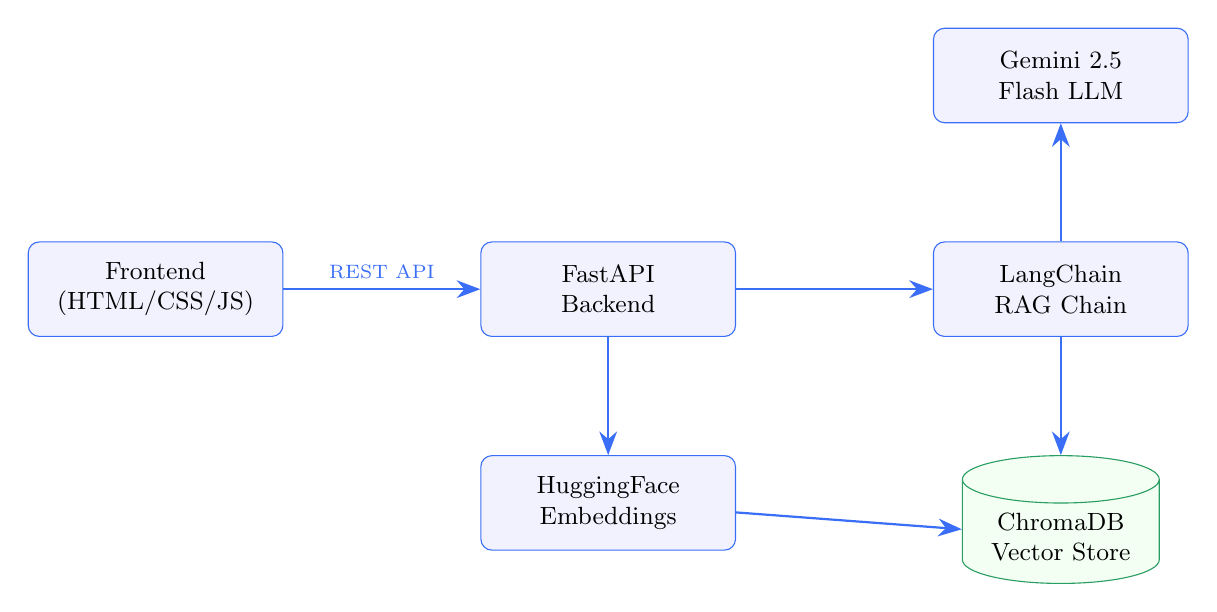
\begin{tikzpicture}[
    node distance=1.5cm and 2.5cm,
    block/.style={rectangle, draw=accentblue, fill=blue!5, text width=3cm,
                  minimum height=1.2cm, align=center, rounded corners=4pt,
                  font=\small},
    db/.style={cylinder, draw=darkgreen, fill=green!5, shape border rotate=90,
               aspect=0.3, minimum width=2.5cm, minimum height=1.2cm,
               align=center, font=\small},
    arrow/.style={-{Stealth[length=3mm]}, thick, accentblue},
  ]

  \node[block] (frontend) {Frontend\\(HTML/CSS/JS)};
  \node[block, right=of frontend] (fastapi) {FastAPI\\Backend};
  \node[block, right=of fastapi] (langchain) {LangChain\\RAG Chain};
  \node[db, below=of langchain] (chromadb) {ChromaDB\\Vector Store};
  \node[block, above=of langchain] (gemini) {Gemini 2.5\\Flash LLM};
  \node[block, below=of fastapi] (embed) {HuggingFace\\Embeddings};

  \draw[arrow] (frontend) -- node[above, font=\scriptsize]{REST API} (fastapi);
  \draw[arrow] (fastapi) -- (langchain);
  \draw[arrow] (langchain) -- (gemini);
  \draw[arrow] (langchain) -- (chromadb);
  \draw[arrow] (embed) -- (chromadb);
  \draw[arrow] (fastapi) -- (embed);
\end{tikzpicture}
\end{center}

\subsection{Component Breakdown}

\begin{longtable}{@{}p{3.5cm}p{4cm}p{6cm}@{}}
\toprule
\textbf{Component} & \textbf{Technology} & \textbf{Purpose} \\
\midrule
\endhead
Frontend & Vanilla HTML/CSS/JS & User interface: file upload, preview, chat \\
Backend API & FastAPI (Python) & REST endpoints, session management, file processing \\
Document Loaders & LangChain Community & Parse PDF, DOCX, PPTX, TXT into text \\
Text Splitter & RecursiveCharacterTextSplitter & Chunk documents (500 chars, 50 overlap) \\
Embeddings & HuggingFace \texttt{all-MiniLM-L6-v2} & Convert text to 384-dim vectors \\
Vector Database & ChromaDB & Store and retrieve embeddings via similarity search \\
LLM & Google Gemini 2.5 Flash & Generate answers from retrieved context \\
Prompt Template & LangChain ChatPromptTemplate & Structure system/user/history messages \\
Conversation Memory & In-memory Python list & Store \texttt{HumanMessage}/\texttt{AIMessage} objects \\
\bottomrule
\end{longtable}

%══════════════════════════════════════════════════════════════════════════════
\section{The RAG Pipeline — Deep Dive}
%══════════════════════════════════════════════════════════════════════════════

RAG (Retrieval-Augmented Generation) is the core architectural pattern of this project. It augments the LLM's generation with relevant retrieved context, reducing hallucination and grounding responses in the user's own documents.

\subsection{Step 1 — Document Ingestion}

When a user uploads files via the \texttt{/upload/\{session\_id\}} endpoint:

\begin{enumerate}
  \item \textbf{Temp File Creation:} Each uploaded file is written to a temporary file on disk (using Python's \texttt{tempfile.NamedTemporaryFile}).
  \item \textbf{Format-Specific Loading:} The correct LangChain loader is selected based on file extension:
    \begin{itemize}
      \item \texttt{.pdf} → \texttt{PyPDFLoader}
      \item \texttt{.docx} → \texttt{UnstructuredWordDocumentLoader}
      \item \texttt{.pptx} → \texttt{UnstructuredPowerPointLoader}
      \item \texttt{.txt} → \texttt{TextLoader}
    \end{itemize}
  \item \textbf{Text Extraction:} Each loader returns a list of \texttt{Document} objects containing \texttt{page\_content} and \texttt{metadata}.
  \item \textbf{Cleanup:} The temporary file is deleted via \texttt{os.unlink()}.
\end{enumerate}

\begin{lstlisting}[language=Python, caption={Document loading logic in main.py}]
def load_file(path: str, ext: str):
    loaders = {
        ".pdf":  PyPDFLoader,
        ".docx": UnstructuredWordDocumentLoader,
        ".pptx": UnstructuredPowerPointLoader,
        ".txt":  TextLoader,
    }
    loader_cls = loaders.get(ext)
    if not loader_cls:
        raise ValueError(f"Unsupported file type: {ext}")
    return loader_cls(path).load()
\end{lstlisting}

\subsection{Step 2 — Text Chunking}

Documents are split into overlapping chunks using \texttt{RecursiveCharacterTextSplitter}:

\begin{itemize}
  \item \textbf{Chunk Size:} 500 characters
  \item \textbf{Chunk Overlap:} 50 characters
  \item \textbf{Why Recursive?} It tries to split by paragraphs → sentences → words → characters, preserving semantic coherence.
  \item \textbf{Why Overlap?} Ensures context at chunk boundaries is not lost.
\end{itemize}

\begin{lstlisting}[language=Python, caption={Text splitter configuration}]
TEXT_SPLITTER = RecursiveCharacterTextSplitter(
    chunk_size=500,
    chunk_overlap=50
)
chunks = TEXT_SPLITTER.split_documents(all_docs)
\end{lstlisting}

\subsection{Step 3 — Embedding Generation}

Each chunk is embedded using the \texttt{all-MiniLM-L6-v2} model from Sentence Transformers:

\begin{itemize}
  \item \textbf{Model:} \texttt{sentence-transformers/all-MiniLM-L6-v2}
  \item \textbf{Embedding Dimension:} 384
  \item \textbf{Why This Model?} Lightweight (22M parameters), fast inference, good semantic quality for retrieval tasks. Runs locally without GPU.
  \item \textbf{Singleton Pattern:} The embedding model is loaded once and cached globally to avoid repeated initialization overhead.
\end{itemize}

\begin{lstlisting}[language=Python, caption={Embedding initialization with caching}]
EMBEDDINGS = None
EMBEDDINGS_ERROR = None

def get_embeddings():
    global EMBEDDINGS, EMBEDDINGS_ERROR
    if EMBEDDINGS is not None:
        return EMBEDDINGS
    if EMBEDDINGS_ERROR is not None:
        raise EMBEDDINGS_ERROR
    try:
        EMBEDDINGS = HuggingFaceEmbeddings(
            model_name="sentence-transformers/all-MiniLM-L6-v2"
        )
        return EMBEDDINGS
    except Exception as exc:
        EMBEDDINGS_ERROR = exc
        raise
\end{lstlisting}

\subsection{Step 4 — Vector Storage (ChromaDB)}

Embeddings are stored in ChromaDB, a lightweight, in-memory vector database:

\begin{itemize}
  \item \textbf{Per-Session Stores:} Each session gets its own ChromaDB collection, ensuring data isolation.
  \item \textbf{Additive Uploads:} If a session already has a vector store, new chunks are appended via \texttt{add\_texts()}.
  \item \textbf{First Upload:} Creates a new collection via \texttt{Chroma.from\_documents()}.
\end{itemize}

\begin{lstlisting}[language=Python, caption={Vector store creation/update}]
if session_id in session_vectorstores:
    session_vectorstores[session_id].add_texts(
        [c.page_content for c in chunks]
    )
else:
    session_vectorstores[session_id] = Chroma.from_documents(
        chunks, embeddings
    )
\end{lstlisting}

\subsection{Step 5 — Retrieval}

When the user asks a question via the \texttt{/ask} endpoint:

\begin{enumerate}
  \item The vector store is converted to a \textbf{retriever} with \texttt{k=4}.
  \item The user's question is embedded using the same \texttt{all-MiniLM-L6-v2} model.
  \item ChromaDB performs a \textbf{cosine similarity search} and returns the top 4 most relevant chunks.
\end{enumerate}

\begin{lstlisting}[language=Python, caption={Retrieval}]
retriever = session_vectorstores[sid].as_retriever(
    search_kwargs={"k": 4}
)
retrieved_docs = retriever.invoke(req.question)
context = format_docs(retrieved_docs)
\end{lstlisting}

\subsection{Step 6 — Prompt Construction \& Generation}

The retrieved context, chat history, and user question are assembled into a structured prompt:

\begin{lstlisting}[language=Python, caption={RAG prompt template}]
RAG_PROMPT = ChatPromptTemplate.from_messages([
    (
        "system",
        """You are a helpful study assistant. Answer questions
using ONLY the context below.
If the answer isn't in the context, say so honestly.

Context:
{context}""",
    ),
    MessagesPlaceholder(variable_name="chat_history"),
    ("human", "{question}"),
])
\end{lstlisting}

The chain is: \texttt{RAG\_PROMPT → Gemini LLM → StrOutputParser}

\begin{lstlisting}[language=Python, caption={Chain execution}]
chain = RAG_PROMPT | llm | StrOutputParser()
answer = chain.invoke({
    "context": context,
    "chat_history": history,
    "question": req.question,
})
\end{lstlisting}

\subsection{Step 7 — Conversation Memory Management}

\begin{itemize}
  \item Each user message is stored as \texttt{HumanMessage} and each AI response as \texttt{AIMessage}.
  \item History is \textbf{truncated to 20 messages} (10 turns) to prevent token overflow.
  \item The \texttt{MessagesPlaceholder} in the prompt template injects the full history into each subsequent call.
\end{itemize}

\begin{lstlisting}[language=Python, caption={History management}]
session_histories[sid].append(HumanMessage(content=req.question))
session_histories[sid].append(AIMessage(content=answer))

# Keep last 20 messages (10 turns)
if len(session_histories[sid]) > 20:
    session_histories[sid] = session_histories[sid][-20:]
\end{lstlisting}

%══════════════════════════════════════════════════════════════════════════════
\section{Backend — FastAPI Deep Dive}
%══════════════════════════════════════════════════════════════════════════════

\subsection{API Endpoints Summary}

\begin{longtable}{@{}p{1.5cm}p{4.5cm}p{7.5cm}@{}}
\toprule
\textbf{Method} & \textbf{Endpoint} & \textbf{Description} \\
\midrule
\endhead
POST & \texttt{/session/new} & Create a new session; returns \texttt{session\_id} \\
POST & \texttt{/upload/\{session\_id\}} & Upload files (multipart); returns chunk count \\
POST & \texttt{/ask} & Ask a question (JSON body); returns RAG answer \\
POST & \texttt{/summarize} & Summarize a specific uploaded file \\
DELETE & \texttt{/session/\{session\_id\}/history} & Clear chat history for a session \\
GET & \texttt{/session/\{session\_id\}} & Get session info (files, history, vectorstore status) \\
GET & \texttt{/health} & Health check endpoint \\
\bottomrule
\end{longtable}

\subsection{Session Management}

The application uses four in-memory dictionaries to manage session state:

\begin{lstlisting}[language=Python, caption={Session state stores}]
session_vectorstores: dict[str, Chroma] = {}    # Vector DBs
session_histories:    dict[str, list]   = {}    # Chat history
session_files:        dict[str, list[str]] = {} # Uploaded filenames
session_docs:         dict[str, dict[str, str]] = {} # Full text for summarization
\end{lstlisting}

\begin{notebox}
In production, these should be replaced with Redis or a proper session store for persistence and horizontal scaling.
\end{notebox}

\subsection{CORS Configuration}

\begin{lstlisting}[language=Python, caption={CORS middleware}]
app.add_middleware(
    CORSMiddleware,
    allow_origins=["*"],   # tighten in production
    allow_methods=["*"],
    allow_headers=["*"],
)
\end{lstlisting}

This allows the frontend (served as a static HTML file via \texttt{file://} or any origin) to communicate with the FastAPI backend.

\subsection{Pydantic Request/Response Models}

\begin{lstlisting}[language=Python, caption={API models}]
class AskRequest(BaseModel):
    session_id: str
    question: str
    gemini_api_key: str

class AskResponse(BaseModel):
    answer: str
    session_id: str
    sources_used: int

class SummarizeRequest(BaseModel):
    session_id: str
    filename: str
    gemini_api_key: str
\end{lstlisting}

\subsection{Error Handling Strategy}

\begin{itemize}
  \item \textbf{404:} Session not found (invalid or expired \texttt{session\_id}).
  \item \textbf{400:} No documents loaded, or no files could be parsed.
  \item \textbf{503:} Embedding model failed to initialize (e.g., missing \texttt{sentence-transformers}).
  \item \textbf{500:} LLM/Summarization errors caught and returned with details.
  \item Unsupported file types return an inline error response (not an HTTP error).
\end{itemize}

%══════════════════════════════════════════════════════════════════════════════
\section{Frontend — UI Deep Dive}
%══════════════════════════════════════════════════════════════════════════════

The frontend is a single \texttt{index.html} file (534 lines) containing all HTML, CSS, and JavaScript.

\subsection{Layout}
\begin{itemize}
  \item \textbf{Top Navigation Bar:} Logo, API key input, Connect button, connection status indicator.
  \item \textbf{Sidebar (260px):} File upload zone (drag-and-drop + click), uploaded file list with type badges.
  \item \textbf{Main Viewer:} Displays file previews (PDF via \texttt{<iframe>}, TXT via \texttt{FileReader}).
  \item \textbf{Chat Panel:} Floating chat window (FAB button), message bubbles, typing indicators.
\end{itemize}

\subsection{Design System}
\begin{itemize}
  \item \textbf{CSS Custom Properties:} 14 design tokens (colors, radii, shadows) defined in \texttt{:root}.
  \item \textbf{Dark Mode:} Automatic via \texttt{@media (prefers-color-scheme: dark)}.
  \item \textbf{Responsive:} CSS Grid layout (\texttt{grid-template-columns: 260px 1fr}).
\end{itemize}

\subsection{Key JavaScript Functions}

\begin{longtable}{@{}p{4cm}p{9.5cm}@{}}
\toprule
\textbf{Function} & \textbf{Purpose} \\
\midrule
\endhead
\texttt{initSession()} & Reads API key, calls \texttt{/session/new}, updates connection status \\
\texttt{uploadFiles()} & Sends files via FormData to \texttt{/upload/\{sid\}}, updates file list \\
\texttt{selectFile(i)} & Renders file preview (PDF iframe / TXT reader / info card) \\
\texttt{sendMessage()} & Posts question to \texttt{/ask}, displays answer bubble \\
\texttt{summarizeFile()} & Calls \texttt{/summarize}, displays summary overlay \\
\texttt{clearHistory()} & DELETE request to clear conversation memory \\
\texttt{toggleChat()} & Shows/hides the floating chat window \\
\bottomrule
\end{longtable}

%══════════════════════════════════════════════════════════════════════════════
\section{Technology Stack — Detailed}
%══════════════════════════════════════════════════════════════════════════════

\subsection{FastAPI}
\begin{itemize}
  \item Modern, async-capable Python web framework.
  \item Automatic OpenAPI/Swagger documentation at \texttt{/docs}.
  \item Built-in request validation via Pydantic.
  \item ASGI server (Uvicorn) for high concurrency.
\end{itemize}

\subsection{LangChain}
\begin{itemize}
  \item Framework for building LLM-powered applications.
  \item Provides abstractions for: document loading, text splitting, embeddings, vector stores, prompts, chains.
  \item Uses LCEL (LangChain Expression Language): \texttt{prompt | llm | parser}.
  \item Sub-packages used: \texttt{langchain-community}, \texttt{langchain-huggingface}, \texttt{langchain-chroma}, \texttt{langchain-google-genai}.
\end{itemize}

\subsection{ChromaDB}
\begin{itemize}
  \item Open-source, lightweight embedding database.
  \item Default: in-memory storage (ephemeral).
  \item Supports cosine, L2, and inner-product distance metrics.
  \item In this project: in-memory, per-session collections.
\end{itemize}

\subsection{Google Gemini 2.5 Flash}
\begin{itemize}
  \item Google's latest multimodal LLM.
  \item Large context window (up to 1M tokens).
  \item Fast inference, cost-effective for production.
  \item Accessed via \texttt{langchain-google-genai} with user-provided API key.
  \item Temperature set to 0.2 for factual, less creative responses.
\end{itemize}

\subsection{HuggingFace Sentence Transformers}
\begin{itemize}
  \item \texttt{all-MiniLM-L6-v2}: 22M parameters, 384-dim embeddings.
  \item Trained on 1B+ sentence pairs for semantic similarity.
  \item Runs locally (no API key needed), CPU-friendly.
  \item Produces normalized embeddings suitable for cosine similarity.
\end{itemize}

\subsection{Dependencies (requirements.txt)}

\begin{longtable}{@{}p{4.5cm}p{9cm}@{}}
\toprule
\textbf{Package} & \textbf{Purpose} \\
\midrule
\endhead
\texttt{fastapi} & Web framework \\
\texttt{uvicorn[standard]} & ASGI server \\
\texttt{python-multipart} & File upload support in FastAPI \\
\texttt{langchain} & Core LangChain framework \\
\texttt{langchain-community} & Document loaders (PDF, DOCX, PPTX, TXT) \\
\texttt{langchain-huggingface} & HuggingFace embeddings integration \\
\texttt{langchain-chroma} & ChromaDB vector store integration \\
\texttt{langchain-google-genai} & Google Gemini LLM integration \\
\texttt{sentence-transformers} & Underlying embedding model \\
\texttt{pypdf} & PDF text extraction \\
\texttt{unstructured} & DOCX/PPTX parsing engine \\
\texttt{python-docx} & Word document support \\
\texttt{python-pptx} & PowerPoint support \\
\texttt{chromadb} & Vector database \\
\bottomrule
\end{longtable}

%══════════════════════════════════════════════════════════════════════════════
\section{Testing}
%══════════════════════════════════════════════════════════════════════════════

The project includes a test file \texttt{test\_main.py} using \texttt{pytest} and FastAPI's \texttt{TestClient}.

\begin{lstlisting}[language=Python, caption={Test: embedding failure returns 503}]
def test_embeddings_failure_returns_503_on_upload(client):
    with patch("main.get_embeddings",
               side_effect=RuntimeError("offline")):
        response = client.post("/session/new", json={})
        sid = response.json()["session_id"]

        upload_response = client.post(
            f"/upload/{sid}",
            files=[("files",
                    ("sample.txt", b"hello world", "text/plain"))],
        )

    assert upload_response.status_code == 503
    assert "Embedding model" in upload_response.json()["detail"]
\end{lstlisting}

\textbf{What this tests:}
\begin{itemize}
  \item Verifies that when the embedding model fails to load, the upload endpoint returns HTTP 503 (Service Unavailable).
  \item Uses \texttt{unittest.mock.patch} to simulate the failure.
  \item Validates both the status code and the error message.
\end{itemize}

%══════════════════════════════════════════════════════════════════════════════
\section{Project Structure}
%══════════════════════════════════════════════════════════════════════════════

\begin{lstlisting}[language=bash, caption={Directory structure}]
Document-AI-Chatbot/
  main.py              # FastAPI backend + RAG logic (316 lines)
  index.html           # Frontend SPA (534 lines)
  requirements.txt     # Python dependencies (14 packages)
  test_main.py         # Pytest unit tests
  README.md            # Project documentation
  .gitignore           # Git ignore rules
  .venv/               # Virtual environment (not committed)
\end{lstlisting}

%══════════════════════════════════════════════════════════════════════════════
\section{How to Run}
%══════════════════════════════════════════════════════════════════════════════

\begin{enumerate}
  \item \textbf{Clone:}
    \begin{lstlisting}[language=bash]
git clone https://github.com/mani30mk/Document-AI-Chatbot.git
cd Document-AI-Chatbot
    \end{lstlisting}

  \item \textbf{Virtual environment:}
    \begin{lstlisting}[language=bash]
python -m venv .venv
.venv\Scripts\Activate.ps1     # Windows PowerShell
    \end{lstlisting}

  \item \textbf{Install dependencies:}
    \begin{lstlisting}[language=bash]
pip install -r requirements.txt
    \end{lstlisting}

  \item \textbf{Start backend:}
    \begin{lstlisting}[language=bash]
uvicorn main:app --reload --port 8000
    \end{lstlisting}

  \item \textbf{Open frontend:} Double-click \texttt{index.html} in your browser. Enter your Gemini API key and click ``Connect''.
\end{enumerate}

%══════════════════════════════════════════════════════════════════════════════
%══════════════════════════════════════════════════════════════════════════════
\newpage
\section{Interview Questions \& Answers}
%══════════════════════════════════════════════════════════════════════════════
%══════════════════════════════════════════════════════════════════════════════

This section contains 50+ interview questions organized by topic. Each question includes a detailed, interview-ready answer.

%──────────────────────────────────────────────────────────────────────────────
\subsection{General Project Questions}
%──────────────────────────────────────────────────────────────────────────────

\begin{interviewbox}[Q1: Can you give a brief overview of your project?]
\end{interviewbox}
\begin{answerbox}
Document AI Chatbot is a full-stack Retrieval-Augmented Generation (RAG) application. Users upload study documents (PDF, DOCX, PPTX, TXT), which are parsed, chunked into 500-character segments with 50-character overlap, embedded using HuggingFace's all-MiniLM-L6-v2 model (384 dimensions), and stored in per-session ChromaDB vector stores. When a user asks a question, the system retrieves the top-4 most semantically similar chunks via cosine similarity, injects them as context into a structured prompt, and sends it to Google Gemini 2.5 Flash for answer generation. The backend is built with FastAPI and LangChain, and the frontend is a single-page HTML/CSS/JS application with a floating chat widget.
\end{answerbox}

\begin{interviewbox}[Q2: Why did you choose RAG over fine-tuning?]
\end{interviewbox}
\begin{answerbox}
Fine-tuning requires retraining the model on domain-specific data, which is expensive, time-consuming, and inflexible—every time new documents are added, you'd need to retrain. RAG, on the other hand, decouples knowledge from the model: the LLM stays general-purpose while document-specific knowledge is stored in a vector database that can be updated instantly. RAG also provides \textbf{traceability}—I can show which chunks were used to generate an answer—and \textbf{reduces hallucination} by grounding responses in actual document content. For a study assistant where documents change frequently, RAG is the clear choice.
\end{answerbox}

\begin{interviewbox}[Q3: What real-world problem does this solve?]
\end{interviewbox}
\begin{answerbox}
Students and professionals often need to extract specific information from large documents quickly. Traditional keyword search misses semantic meaning (e.g., searching ``salary'' won't find ``compensation'' or ``remuneration''). This project uses semantic vector search to understand meaning, not just keywords, and generates natural-language answers. It's like having a personal tutor who has read all your materials and can answer questions with context.
\end{answerbox}

\begin{interviewbox}[Q4: What are the limitations of your current implementation?]
\end{interviewbox}
\begin{answerbox}
\begin{enumerate}
  \item \textbf{In-memory state:} Sessions are lost on server restart (no persistence).
  \item \textbf{No authentication:} Any user can create sessions; API keys are sent in plain JSON.
  \item \textbf{Single-server:} In-memory dicts can't scale horizontally.
  \item \textbf{No streaming:} Answers come as a single response (no token-by-token streaming).
  \item \textbf{CORS wildcard:} \texttt{allow\_origins=["*"]} is too permissive for production.
  \item \textbf{Fixed chunk parameters:} 500-char chunks may not be optimal for all document types.
  \item \textbf{No re-ranking:} Retrieved chunks aren't re-ranked before being sent to the LLM.
\end{enumerate}
\end{answerbox}

\begin{interviewbox}[Q5: How would you deploy this to production?]
\end{interviewbox}
\begin{answerbox}
\begin{enumerate}
  \item \textbf{Backend:} Containerize with Docker, deploy on AWS ECS / GCP Cloud Run / Kubernetes.
  \item \textbf{Session State:} Replace in-memory dicts with Redis for persistence and horizontal scaling.
  \item \textbf{Vector DB:} Switch from in-memory ChromaDB to a managed service like Pinecone, Weaviate, or persistent ChromaDB with a disk-backed SQLite.
  \item \textbf{Frontend:} Serve via CDN (CloudFront, Vercel).
  \item \textbf{Security:} Add OAuth2/JWT authentication; store API keys server-side encrypted; restrict CORS origins.
  \item \textbf{Monitoring:} Add LangSmith for LLM observability, Prometheus/Grafana for metrics.
  \item \textbf{Streaming:} Use Server-Sent Events (SSE) or WebSockets for token-by-token responses.
\end{enumerate}
\end{answerbox}

%──────────────────────────────────────────────────────────────────────────────
\subsection{RAG \& LangChain Questions}
%──────────────────────────────────────────────────────────────────────────────

\begin{interviewbox}[Q6: Explain the RAG pipeline step by step.]
\end{interviewbox}
\begin{answerbox}
\begin{enumerate}
  \item \textbf{Ingestion:} Documents are uploaded and parsed using format-specific LangChain loaders (PyPDFLoader, UnstructuredWordDocumentLoader, etc.).
  \item \textbf{Chunking:} Text is split into 500-character chunks with 50-character overlap using RecursiveCharacterTextSplitter.
  \item \textbf{Embedding:} Each chunk is converted to a 384-dimensional vector using the all-MiniLM-L6-v2 sentence transformer model.
  \item \textbf{Storage:} Vectors are stored in a per-session ChromaDB collection.
  \item \textbf{Retrieval:} When a user asks a question, the question is embedded using the same model, and the top-4 most similar chunks are retrieved via cosine similarity.
  \item \textbf{Augmentation:} Retrieved chunks are formatted and injected into the system prompt as ``Context''.
  \item \textbf{Generation:} The full prompt (system + context + chat history + question) is sent to Gemini 2.5 Flash, which generates a grounded answer.
\end{enumerate}
\end{answerbox}

\begin{interviewbox}[Q7: Why did you use RecursiveCharacterTextSplitter instead of other splitters?]
\end{interviewbox}
\begin{answerbox}
\texttt{RecursiveCharacterTextSplitter} is the most versatile splitter because it uses a hierarchy of separators: \texttt{["\textbackslash n\textbackslash n", "\textbackslash n", " ", ""]}. It first tries to split by double newlines (paragraphs), then single newlines, then spaces, then individual characters. This preserves semantic boundaries as much as possible within the chunk size constraint. Alternatives like \texttt{CharacterTextSplitter} only split on a single separator, which can break mid-sentence. \texttt{TokenTextSplitter} is token-based (useful for precise token budgets) but slower. For a general-purpose study assistant handling diverse document types, \texttt{RecursiveCharacterTextSplitter} offers the best balance.
\end{answerbox}

\begin{interviewbox}[Q8: Why chunk size 500 and overlap 50? How would you tune these?]
\end{interviewbox}
\begin{answerbox}
\textbf{500 characters} is approximately 100--125 tokens—small enough to be semantically focused but large enough to contain a complete thought. \textbf{50-character overlap} ensures that information at chunk boundaries isn't lost. To tune:
\begin{itemize}
  \item \textbf{Increase chunk size} (1000+) for documents with long, cohesive paragraphs (e.g., legal contracts).
  \item \textbf{Decrease chunk size} (200--300) for FAQ-style or highly structured content.
  \item \textbf{Evaluate empirically:} Use retrieval metrics like precision@k, recall@k, or MRR (Mean Reciprocal Rank) on a test set.
  \item Consider \textbf{semantic chunking} (splitting by topic/meaning) for more advanced use cases.
\end{itemize}
\end{answerbox}

\begin{interviewbox}[Q9: What is LCEL and how does your project use it?]
\end{interviewbox}
\begin{answerbox}
LCEL (LangChain Expression Language) is a declarative way to compose LangChain components using the pipe (\texttt{|}) operator. In my project, the chain is:

\texttt{RAG\_PROMPT | llm | StrOutputParser()}

This means: take the prompt template, pass its output to the LLM, then parse the LLM's output to a plain string. LCEL supports streaming, batching, and async out of the box. It replaces the older \texttt{LLMChain} and \texttt{SequentialChain} patterns.
\end{answerbox}

\begin{interviewbox}[Q10: How does the conversation memory work?]
\end{interviewbox}
\begin{answerbox}
I use a manual list-based approach with LangChain's \texttt{HumanMessage} and \texttt{AIMessage} objects. After each Q\&A turn:
\begin{enumerate}
  \item The question is appended as a \texttt{HumanMessage}.
  \item The answer is appended as an \texttt{AIMessage}.
  \item If the history exceeds 20 messages (10 turns), the oldest messages are trimmed.
\end{enumerate}
The history is injected into the prompt via \texttt{MessagesPlaceholder(variable\_name="chat\_history")}. This lets the LLM understand follow-up questions like ``What about the second point?'' by seeing the prior conversation context.
\end{answerbox}

\begin{interviewbox}[Q11: Why top-k=4 for retrieval? How would you improve retrieval quality?]
\end{interviewbox}
\begin{answerbox}
\textbf{k=4} is a practical default—enough context for most questions without overwhelming the LLM or exceeding token limits. To improve retrieval:
\begin{enumerate}
  \item \textbf{Re-ranking:} Use a cross-encoder model (e.g., \texttt{ms-marco-MiniLM}) to re-rank the top-20 retrieved chunks and select the best 4.
  \item \textbf{Hybrid search:} Combine dense (vector) retrieval with sparse (BM25/TF-IDF) retrieval for better keyword coverage.
  \item \textbf{MMR (Maximal Marginal Relevance):} Diversify results to avoid redundant chunks: \texttt{search\_type="mmr"}.
  \item \textbf{Metadata filtering:} Filter chunks by source file or page number.
  \item \textbf{Query expansion:} Use the LLM to generate multiple query reformulations before retrieval.
\end{enumerate}
\end{answerbox}

\begin{interviewbox}[Q12: Explain what cosine similarity is and why it's used for retrieval.]
\end{interviewbox}
\begin{answerbox}
Cosine similarity measures the angle between two vectors in a high-dimensional space:

$$\text{cosine\_sim}(A, B) = \frac{A \cdot B}{\|A\| \times \|B\|}$$

It ranges from $-1$ (opposite) to $1$ (identical direction). It's used for retrieval because:
\begin{itemize}
  \item It's \textbf{magnitude-invariant}: only considers the direction (meaning), not the length of the vector.
  \item Semantically similar texts produce vectors pointing in similar directions, regardless of document length.
  \item The all-MiniLM-L6-v2 model produces normalized embeddings, so cosine similarity simplifies to a dot product—very fast to compute.
\end{itemize}
\end{answerbox}

\begin{interviewbox}[Q13: What is the difference between an embedding and a vector?]
\end{interviewbox}
\begin{answerbox}
A \textbf{vector} is a general mathematical object—an ordered list of numbers. An \textbf{embedding} is a specific type of vector that is the \textit{learned representation} of data (text, images, etc.) in a continuous vector space, where semantic similarity maps to geometric proximity. In this project, each text chunk is converted to a 384-dimensional embedding where chunks about similar topics end up close together in vector space.
\end{answerbox}

\begin{interviewbox}[Q14: How does the system prompt prevent hallucination?]
\end{interviewbox}
\begin{answerbox}
The system prompt explicitly instructs: ``\textit{Answer questions using ONLY the context below. If the answer isn't in the context, say so honestly.}'' This is a \textbf{grounding constraint}—it tells the LLM to use only the retrieved context, not its pretrained knowledge. When the answer isn't in the retrieved chunks, the model is instructed to admit it rather than fabricate an answer. This is a key RAG pattern called ``faithfulness to context.''
\end{answerbox}

\begin{interviewbox}[Q15: What happens if no relevant chunks are found?]
\end{interviewbox}
\begin{answerbox}
ChromaDB always returns exactly $k$ results regardless of relevance scores—there's no built-in threshold. So even for an unrelated question, 4 chunks are returned. However:
\begin{enumerate}
  \item The system prompt says ``if the answer isn't in the context, say so honestly,'' so the LLM should respond appropriately.
  \item To improve this, I could add a \textbf{relevance score threshold}: filter out chunks with cosine similarity below, say, 0.3, and if no chunks pass the threshold, return a message like ``I couldn't find relevant information in your documents.''
\end{enumerate}
\end{answerbox}

%──────────────────────────────────────────────────────────────────────────────
\subsection{FastAPI \& Backend Questions}
%──────────────────────────────────────────────────────────────────────────────

\begin{interviewbox}[Q16: Why FastAPI over Flask or Django?]
\end{interviewbox}
\begin{answerbox}
\begin{enumerate}
  \item \textbf{Async-native:} FastAPI is built on ASGI (Starlette), supporting \texttt{async/await} natively—critical for I/O-bound operations like LLM API calls.
  \item \textbf{Automatic validation:} Pydantic models validate request bodies, query parameters, and path parameters with zero boilerplate.
  \item \textbf{Auto-generated docs:} Swagger UI at \texttt{/docs} and ReDoc at \texttt{/redoc} are generated automatically from type hints.
  \item \textbf{Performance:} One of the fastest Python frameworks, comparable to Go/Node.js for I/O-bound tasks.
  \item Flask lacks native async support and requires extensions for validation. Django is heavy for a microservice.
\end{enumerate}
\end{answerbox}

\begin{interviewbox}[Q17: Explain how file upload works in your backend.]
\end{interviewbox}
\begin{answerbox}
The \texttt{/upload/\{session\_id\}} endpoint accepts \texttt{multipart/form-data} using FastAPI's \texttt{UploadFile} type:
\begin{enumerate}
  \item Files arrive as \texttt{List[UploadFile]} via the \texttt{files} form field.
  \item Each file is written to a \textbf{temporary file} using \texttt{tempfile.NamedTemporaryFile} because LangChain loaders require a file path (they can't read from memory).
  \item The appropriate loader is selected based on file extension.
  \item After loading, the temp file is \textbf{deleted} via \texttt{os.unlink()} in a \texttt{finally} block to ensure cleanup even if parsing fails.
  \item The full text is stored in \texttt{session\_docs} for the summarization feature.
\end{enumerate}
\end{answerbox}

\begin{interviewbox}[Q18: Why use \texttt{tempfile} instead of reading files directly into memory?]
\end{interviewbox}
\begin{answerbox}
LangChain document loaders (PyPDFLoader, UnstructuredWordDocumentLoader, etc.) are designed to accept \textbf{file paths}, not file objects or byte streams. They internally open the file from disk. So we must write the uploaded bytes to a temporary file, let the loader read it, and then clean up. An alternative would be to write custom loaders that accept byte streams, but using \texttt{tempfile} is simpler and leverages the existing, well-tested loader ecosystem.
\end{answerbox}

\begin{interviewbox}[Q19: What is CORS and why is it needed here?]
\end{interviewbox}
\begin{answerbox}
CORS (Cross-Origin Resource Sharing) is a browser security mechanism that blocks web pages from making requests to a different origin (domain/port). Since the frontend is served from \texttt{file://} or a different port (not 8000), the browser would block API calls to \texttt{http://localhost:8000} without CORS headers. The middleware adds headers like \texttt{Access-Control-Allow-Origin: *} to tell the browser it's safe to proceed. In production, I'd restrict \texttt{allow\_origins} to the specific frontend domain.
\end{answerbox}

\begin{interviewbox}[Q20: How does session management work? What are its weaknesses?]
\end{interviewbox}
\begin{answerbox}
Sessions are managed via four Python dictionaries keyed by UUID. When \texttt{/session/new} is called, a UUID is generated and used as the session ID. All subsequent operations (upload, ask, summarize) require this session ID. \textbf{Weaknesses:}
\begin{itemize}
  \item \textbf{No persistence:} Server restart loses all sessions.
  \item \textbf{No expiration:} Sessions never expire, causing memory leaks.
  \item \textbf{No horizontal scaling:} In-memory state can't be shared across multiple server instances.
  \item \textbf{No authentication:} Anyone who guesses/intercepts a session ID can access it.
\end{itemize}
\textbf{Fix:} Use Redis with TTL-based expiration, JWT tokens for auth, and persistent vector DBs like Pinecone.
\end{answerbox}

\begin{interviewbox}[Q21: What is Pydantic and how do you use it?]
\end{interviewbox}
\begin{answerbox}
Pydantic is a data validation library that uses Python type hints to define schemas. In my project, I use Pydantic's \texttt{BaseModel} for:
\begin{itemize}
  \item \texttt{AskRequest}: Validates that \texttt{session\_id}, \texttt{question}, and \texttt{gemini\_api\_key} are all strings.
  \item \texttt{AskResponse}: Ensures the response contains \texttt{answer} (str), \texttt{session\_id} (str), and \texttt{sources\_used} (int).
  \item \texttt{SummarizeRequest}: Validates the summarization request.
\end{itemize}
FastAPI automatically returns a 422 error with details if the request body doesn't match the model. This eliminates manual validation code.
\end{answerbox}

\begin{interviewbox}[Q22: What does \texttt{uvicorn main:app --reload} do?]
\end{interviewbox}
\begin{answerbox}
\texttt{uvicorn} is an ASGI server. \texttt{main:app} tells it to import the \texttt{app} object from \texttt{main.py}. \texttt{--reload} enables auto-reload: the server watches for file changes and restarts automatically (development mode only). \texttt{--port 8000} sets the listening port. In production, you'd remove \texttt{--reload} and use \texttt{--workers N} for multi-process concurrency.
\end{answerbox}

%──────────────────────────────────────────────────────────────────────────────
\subsection{Embeddings \& Vector Database Questions}
%──────────────────────────────────────────────────────────────────────────────

\begin{interviewbox}[Q23: Why all-MiniLM-L6-v2 over OpenAI embeddings?]
\end{interviewbox}
\begin{answerbox}
\begin{enumerate}
  \item \textbf{Free:} No API costs; runs locally.
  \item \textbf{Privacy:} Document content never leaves the user's machine.
  \item \textbf{Fast:} 22M parameters; sub-second inference on CPU.
  \item \textbf{Good quality:} Top performer on sentence similarity benchmarks for its size class.
  \item \textbf{No rate limits:} Unlike OpenAI's API, there are no throttling concerns.
  \item Trade-off: OpenAI's \texttt{text-embedding-3-large} (3072 dims) may capture more nuance, but at the cost of API latency, cost, and privacy.
\end{enumerate}
\end{answerbox}

\begin{interviewbox}[Q24: What is ChromaDB and why did you choose it?]
\end{interviewbox}
\begin{answerbox}
ChromaDB is an open-source vector database designed for AI applications. I chose it because:
\begin{itemize}
  \item \textbf{Zero infrastructure:} Runs in-memory with no external server needed.
  \item \textbf{LangChain integration:} \texttt{langchain-chroma} provides seamless \texttt{from\_documents()} and \texttt{as\_retriever()} methods.
  \item \textbf{Development speed:} Perfect for prototyping without managing a separate database service.
  \item For production, I'd switch to Pinecone (managed, scalable), Weaviate (open-source, production-ready), or Qdrant (high-performance, Rust-based).
\end{itemize}
\end{answerbox}

\begin{interviewbox}[Q25: How does similarity search work internally in ChromaDB?]
\end{interviewbox}
\begin{answerbox}
\begin{enumerate}
  \item The query text is embedded using the same embedding model.
  \item ChromaDB computes the distance (default: L2/Euclidean, but cosine is also supported) between the query embedding and all stored embeddings.
  \item The top-$k$ closest embeddings are returned, along with their associated text chunks and metadata.
  \item For small datasets (thousands of chunks), this is a brute-force comparison. For larger datasets, ChromaDB uses HNSW (Hierarchical Navigable Small World) indexing for approximate nearest neighbor (ANN) search.
\end{enumerate}
\end{answerbox}

\begin{interviewbox}[Q26: What is the Singleton pattern in your embedding initialization?]
\end{interviewbox}
\begin{answerbox}
The \texttt{get\_embeddings()} function implements a lazy singleton: the embedding model is loaded only once on first call and cached in the global \texttt{EMBEDDINGS} variable. Subsequent calls return the cached instance. If loading fails, the error is also cached in \texttt{EMBEDDINGS\_ERROR} to avoid repeated failed initialization attempts. This saves memory and startup time since loading a transformer model involves downloading weights and initializing PyTorch tensors.
\end{answerbox}

%──────────────────────────────────────────────────────────────────────────────
\subsection{LLM \& Gemini Questions}
%──────────────────────────────────────────────────────────────────────────────

\begin{interviewbox}[Q27: Why Gemini 2.5 Flash over GPT-4 or Claude?]
\end{interviewbox}
\begin{answerbox}
\begin{enumerate}
  \item \textbf{Large context window:} Up to 1M tokens—crucial for the summarization feature that sends full document text.
  \item \textbf{Cost-effective:} Flash variant is optimized for speed and cost.
  \item \textbf{Fast inference:} Lower latency than GPT-4.
  \item \textbf{Free tier:} Google offers a generous free tier for Gemini API.
  \item \textbf{Quality:} Competitive with GPT-4 on reasoning and factual tasks.
  \item The architecture is model-agnostic—swapping to GPT-4 or Claude requires only changing the LLM class and API key.
\end{enumerate}
\end{answerbox}

\begin{interviewbox}[Q28: Why temperature 0.2? What happens at 0 vs. 1?]
\end{interviewbox}
\begin{answerbox}
Temperature controls the randomness of token sampling:
\begin{itemize}
  \item \textbf{0 (deterministic):} Always picks the most probable token. Good for factual Q\&A but can be repetitive.
  \item \textbf{0.2 (low):} Mostly deterministic with slight variation—ideal for our use case where we want factual, consistent answers from document context.
  \item \textbf{1.0 (creative):} More diverse, creative outputs—useful for brainstorming or creative writing but undesirable for factual retrieval.
\end{itemize}
For a study assistant, 0.2 ensures the model sticks closely to the retrieved context while maintaining natural language flow.
\end{answerbox}

\begin{interviewbox}[Q29: How does the summarization feature differ from RAG Q\&A?]
\end{interviewbox}
\begin{answerbox}
They are fundamentally different approaches:
\begin{itemize}
  \item \textbf{RAG Q\&A:} Retrieves only top-$k$ relevant chunks → generates an answer from partial context. Uses the vector store and retriever.
  \item \textbf{Summarization:} Sends the \textbf{entire document text} to Gemini in a single prompt. No vector store involved. Leverages Gemini's 1M-token context window to read the full document and produce a cohesive summary.
\end{itemize}
This is why \texttt{session\_docs} stores the full text separately from the chunked vector store.
\end{answerbox}

\begin{interviewbox}[Q30: What is a prompt template and why use one?]
\end{interviewbox}
\begin{answerbox}
A prompt template is a reusable structure that defines how to construct the input to an LLM. In my project, \texttt{ChatPromptTemplate.from\_messages()} creates a multi-message prompt with:
\begin{enumerate}
  \item A \textbf{system message} containing instructions and the retrieved context.
  \item A \textbf{MessagesPlaceholder} for chat history (dynamically injected).
  \item A \textbf{human message} with the current question.
\end{enumerate}
Benefits: consistency across calls, separation of concerns (logic vs. prompt), easy experimentation with different prompts, and type-safe variable injection.
\end{answerbox}

%──────────────────────────────────────────────────────────────────────────────
\subsection{Frontend Questions}
%──────────────────────────────────────────────────────────────────────────────

\begin{interviewbox}[Q31: Why a single HTML file instead of React/Vue?]
\end{interviewbox}
\begin{answerbox}
The frontend is intentionally lightweight:
\begin{itemize}
  \item \textbf{Zero build step:} No npm, Webpack, or bundling—just double-click to open.
  \item \textbf{Instant deployment:} Can be served from any static file server or CDN.
  \item \textbf{Focus on backend:} This is primarily a backend/AI project; the frontend demonstrates the capability without overengineering.
  \item At ~534 lines, the complexity is manageable in a single file.
  \item For a production version, I'd use React or Next.js with proper state management.
\end{itemize}
\end{answerbox}

\begin{interviewbox}[Q32: How does drag-and-drop file upload work?]
\end{interviewbox}
\begin{answerbox}
The upload zone listens for three DOM events:
\begin{enumerate}
  \item \texttt{dragover}: Prevents the browser's default behavior (opening the file) and adds a visual highlight class.
  \item \texttt{dragleave}: Removes the highlight.
  \item \texttt{drop}: Prevents default, extracts files from \texttt{e.dataTransfer.files}, and calls \texttt{uploadFiles()}.
\end{enumerate}
Files are also uploadable via the hidden \texttt{<input type="file">} element triggered by clicking the upload zone (it's wrapped in a \texttt{<label>}).
\end{answerbox}

\begin{interviewbox}[Q33: How does the PDF viewer work?]
\end{interviewbox}
\begin{answerbox}
When a PDF file is selected:
\begin{enumerate}
  \item A \textbf{Blob URL} is created from the original \texttt{File} object using \texttt{URL.createObjectURL(f)}.
  \item This URL is set as the \texttt{src} of an \texttt{<iframe>}.
  \item The browser's native PDF viewer renders the file inside the iframe.
  \item When a file is removed, \texttt{URL.revokeObjectURL()} is called to free memory.
\end{enumerate}
For TXT files, \texttt{FileReader.readAsText()} loads the content and displays it in a \texttt{<div>} with \texttt{white-space: pre-wrap}.
\end{answerbox}

\begin{interviewbox}[Q34: How does the dark mode work?]
\end{interviewbox}
\begin{answerbox}
The CSS uses \texttt{@media (prefers-color-scheme: dark)} to override the \texttt{:root} CSS custom properties when the user's OS is set to dark mode. No JavaScript is involved—it's entirely CSS-driven. The design tokens (colors) are defined as CSS variables, so changing them in the media query automatically updates the entire UI.
\end{answerbox}

%──────────────────────────────────────────────────────────────────────────────
\subsection{Advanced / Design Decision Questions}
%──────────────────────────────────────────────────────────────────────────────

\begin{interviewbox}[Q35: How would you handle very large documents (1000+ pages)?]
\end{interviewbox}
\begin{answerbox}
\begin{enumerate}
  \item \textbf{Async processing:} Move file processing to a background task queue (Celery/RQ). Return immediately with a ``processing'' status and poll for completion.
  \item \textbf{Batch chunking:} Process documents in batches to avoid memory spikes.
  \item \textbf{Streaming upload:} Use chunked file uploads for very large files.
  \item \textbf{Persistent vector store:} Use disk-backed ChromaDB or Pinecone to avoid holding all vectors in memory.
  \item \textbf{Hierarchical summarization:} For summarization, use a map-reduce or refine strategy instead of sending the entire text (which may exceed even Gemini's context window).
\end{enumerate}
\end{answerbox}

\begin{interviewbox}[Q36: How would you add authentication?]
\end{interviewbox}
\begin{answerbox}
\begin{enumerate}
  \item \textbf{JWT Authentication:} Use FastAPI's \texttt{OAuth2PasswordBearer} dependency with JWT tokens.
  \item \textbf{User registration:} Add a \texttt{/auth/register} and \texttt{/auth/login} endpoint.
  \item \textbf{API key security:} Store Gemini API keys encrypted in a database (not sent from the frontend).
  \item \textbf{Session ownership:} Link sessions to authenticated users; reject requests from non-owners.
  \item \textbf{Rate limiting:} Use \texttt{slowapi} middleware to prevent abuse.
\end{enumerate}
\end{answerbox}

\begin{interviewbox}[Q37: How would you add streaming responses?]
\end{interviewbox}
\begin{answerbox}
\begin{enumerate}
  \item Change the LLM to streaming mode: \texttt{llm.stream()} instead of \texttt{llm.invoke()}.
  \item Use FastAPI's \texttt{StreamingResponse} with \texttt{text/event-stream} content type (Server-Sent Events).
  \item On the frontend, use the \texttt{EventSource} API or \texttt{fetch} with \texttt{ReadableStream} to consume tokens as they arrive.
  \item Display tokens incrementally in the chat bubble for a ``typing'' effect.
\end{enumerate}
\end{answerbox}

\begin{interviewbox}[Q38: How would you implement re-ranking?]
\end{interviewbox}
\begin{answerbox}
After retrieving the top-$k$ chunks (e.g., top-20), pass each (query, chunk) pair through a cross-encoder model like \texttt{cross-encoder/ms-marco-MiniLM-L-6-v2}. Cross-encoders jointly encode the query and passage and output a relevance score. Re-rank by this score and take the top-4. This is more accurate than bi-encoder similarity because the cross-encoder can model fine-grained interactions between the query and passage. In LangChain, use \texttt{FlashrankRerank} or \texttt{CohereRerank}.
\end{answerbox}

\begin{interviewbox}[Q39: What is the difference between bi-encoder and cross-encoder?]
\end{interviewbox}
\begin{answerbox}
\begin{itemize}
  \item \textbf{Bi-encoder} (used in this project): Encodes query and document \textit{independently} into vectors, then compares via cosine similarity. Fast (O($n$) for $n$ documents). Used for retrieval.
  \item \textbf{Cross-encoder}: Takes (query, document) as a \textit{single input pair} and outputs a relevance score. More accurate but slow (O($n \times q$) inference). Used for re-ranking a small candidate set.
\end{itemize}
Best practice: Use a bi-encoder to retrieve 20--50 candidates, then a cross-encoder to re-rank and select the top-$k$.
\end{answerbox}

\begin{interviewbox}[Q40: How would you add hybrid search (dense + sparse)?]
\end{interviewbox}
\begin{answerbox}
Hybrid search combines:
\begin{itemize}
  \item \textbf{Dense retrieval:} Vector similarity (what we currently do). Good at semantic/conceptual matching.
  \item \textbf{Sparse retrieval:} BM25/TF-IDF keyword matching. Good at exact term matching (names, codes, acronyms).
\end{itemize}
Implementation: Use \texttt{BM25Retriever} from LangChain alongside the vector retriever, then merge results using \texttt{EnsembleRetriever} with weighted scores (e.g., 0.6 dense + 0.4 sparse). This handles queries where exact keywords matter (e.g., ``What is the FERPA policy?'') better than pure semantic search.
\end{answerbox}

\begin{interviewbox}[Q41: What is Maximal Marginal Relevance (MMR)?]
\end{interviewbox}
\begin{answerbox}
MMR is a retrieval strategy that balances \textbf{relevance} and \textbf{diversity}. Standard top-$k$ retrieval might return 4 chunks that are all semantically similar (redundant). MMR iteratively selects chunks that are:
\begin{enumerate}
  \item Highly relevant to the query.
  \item Dissimilar from already-selected chunks.
\end{enumerate}
The formula:
$$\text{MMR} = \arg\max_{d_i} \left[ \lambda \cdot \text{sim}(d_i, q) - (1-\lambda) \cdot \max_{d_j \in S} \text{sim}(d_i, d_j) \right]$$

In LangChain: \texttt{retriever = vectorstore.as\_retriever(search\_type="mmr")}.
\end{answerbox}

%──────────────────────────────────────────────────────────────────────────────
\subsection{Python \& Software Engineering Questions}
%──────────────────────────────────────────────────────────────────────────────

\begin{interviewbox}[Q42: Why use \texttt{async def} for some endpoints but \texttt{def} for others?]
\end{interviewbox}
\begin{answerbox}
In FastAPI:
\begin{itemize}
  \item \texttt{async def} is used when the function contains \texttt{await} calls (e.g., \texttt{await uf.read()} for file uploads). It runs on the main event loop.
  \item \texttt{def} (synchronous) is used when there are no async operations. FastAPI automatically runs these in a thread pool to avoid blocking the event loop.
\end{itemize}
In my code: \texttt{upload\_files} and \texttt{ask} are async (they use \texttt{await}), while \texttt{new\_session}, \texttt{clear\_history}, \texttt{session\_info}, and \texttt{health} are synchronous (they do simple dict operations).
\end{answerbox}

\begin{interviewbox}[Q43: What is the purpose of the \texttt{finally} block in the upload handler?]
\end{interviewbox}
\begin{answerbox}
The \texttt{finally} block ensures that the temporary file is \textbf{always deleted}, even if the loader throws an exception (e.g., corrupt file, unsupported content). Without it, failed uploads would leave orphan temp files on disk, eventually filling up storage. This is a resource cleanup pattern.

\begin{lstlisting}[language=Python]
try:
    docs = load_file(tmp_path, ext)
except ValueError as e:
    return {"error": str(e), "skipped": uf.filename}
finally:
    os.unlink(tmp_path)  # Always runs
\end{lstlisting}
\end{answerbox}

\begin{interviewbox}[Q44: How do you handle the Gemini API key securely?]
\end{interviewbox}
\begin{answerbox}
\textbf{Currently:} The API key is entered by the user in the browser and sent with each request in the JSON body. This means:
\begin{itemize}
  \item The key is in memory only; it's never stored on the server.
  \item Each user provides their own key—no shared key that could be compromised.
\end{itemize}
\textbf{Security concern:} The key is sent in plaintext over HTTP (not HTTPS in local development). In production:
\begin{itemize}
  \item Enforce HTTPS.
  \item Store keys server-side encrypted in a secrets manager (e.g., AWS Secrets Manager).
  \item Use a server-side API key with per-user rate limiting.
\end{itemize}
\end{answerbox}

\begin{interviewbox}[Q45: What is the \texttt{response\_model} parameter in FastAPI?]
\end{interviewbox}
\begin{answerbox}
\texttt{response\_model} tells FastAPI to:
\begin{enumerate}
  \item \textbf{Validate} the response data against the Pydantic model before sending.
  \item \textbf{Serialize} the response, filtering out any extra fields not in the model.
  \item \textbf{Document} the response schema in the auto-generated OpenAPI spec.
\end{enumerate}
For example, \texttt{@app.post("/ask", response\_model=AskResponse)} ensures the response always contains exactly \texttt{answer}, \texttt{session\_id}, and \texttt{sources\_used}.
\end{answerbox}

%──────────────────────────────────────────────────────────────────────────────
\subsection{Testing \& Quality Questions}
%──────────────────────────────────────────────────────────────────────────────

\begin{interviewbox}[Q46: Explain the test in \texttt{test\_main.py}.]
\end{interviewbox}
\begin{answerbox}
The test verifies that when the embedding model fails to initialize (simulated via \texttt{unittest.mock.patch} making \texttt{get\_embeddings} raise \texttt{RuntimeError("offline")}), the upload endpoint returns:
\begin{itemize}
  \item HTTP status code \textbf{503} (Service Unavailable).
  \item An error message containing ``Embedding model''.
\end{itemize}
This is a \textbf{fault injection test}—it validates that the system handles dependency failures gracefully instead of crashing with a 500 error.
\end{answerbox}

\begin{interviewbox}[Q47: What additional tests would you write?]
\end{interviewbox}
\begin{answerbox}
\begin{enumerate}
  \item \textbf{Session lifecycle:} Create session → upload → ask → verify answer contains expected content.
  \item \textbf{Invalid session:} Ask with a non-existent session ID → expect 404.
  \item \textbf{No files uploaded:} Ask before uploading → expect 400.
  \item \textbf{Unsupported file type:} Upload a \texttt{.exe} file → expect error response.
  \item \textbf{Clear history:} Send messages → clear → verify history is empty.
  \item \textbf{Multiple file upload:} Upload 3 files → verify all are indexed.
  \item \textbf{Chunk count:} Upload a known document → verify expected chunk count.
  \item \textbf{Integration test:} Full RAG pipeline with a mock LLM to verify end-to-end flow.
  \item \textbf{Load test:} Use \texttt{locust} to test concurrent sessions.
\end{enumerate}
\end{answerbox}

\begin{interviewbox}[Q48: How would you evaluate RAG quality?]
\end{interviewbox}
\begin{answerbox}
RAG evaluation has two dimensions:
\begin{itemize}
  \item \textbf{Retrieval quality:}
    \begin{itemize}
      \item Precision@k: What fraction of retrieved chunks are relevant?
      \item Recall@k: What fraction of relevant chunks were retrieved?
      \item MRR (Mean Reciprocal Rank): Where does the first relevant chunk appear?
    \end{itemize}
  \item \textbf{Generation quality:}
    \begin{itemize}
      \item \textbf{Faithfulness:} Does the answer use only the retrieved context? (Use RAGAS framework.)
      \item \textbf{Answer relevance:} Does the answer address the question?
      \item \textbf{Groundedness:} Can every claim in the answer be traced to a source chunk?
    \end{itemize}
  \item \textbf{Tools:} RAGAS, LangSmith evaluations, or custom evaluation pipelines with LLM-as-judge.
\end{itemize}
\end{answerbox}

%──────────────────────────────────────────────────────────────────────────────
\subsection{Scenario-Based Questions}
%──────────────────────────────────────────────────────────────────────────────

\begin{interviewbox}[Q49: A user uploads a 500-page PDF and the app becomes slow. How do you debug and fix this?]
\end{interviewbox}
\begin{answerbox}
\textbf{Diagnosis:}
\begin{enumerate}
  \item Profile the upload endpoint to find the bottleneck: is it file parsing, chunking, embedding, or ChromaDB insertion?
  \item Most likely bottleneck: \textbf{embedding generation}—each chunk requires a forward pass through the transformer model.
\end{enumerate}
\textbf{Fixes:}
\begin{enumerate}
  \item \textbf{Batch embedding:} Embed chunks in batches (e.g., 64 at a time) instead of one by one.
  \item \textbf{GPU acceleration:} Use CUDA-enabled PyTorch for the embedding model.
  \item \textbf{Background processing:} Return immediately and process in a background task queue (Celery). Notify the user when indexing is complete.
  \item \textbf{Progress feedback:} Send Server-Sent Events to the frontend showing ``Indexing: 45/100 chunks...''.
  \item \textbf{Caching:} Hash file content; if the same file was uploaded before, skip re-processing.
\end{enumerate}
\end{answerbox}

\begin{interviewbox}[Q50: The LLM gives wrong answers even though the correct information is in the document. What could be wrong?]
\end{interviewbox}
\begin{answerbox}
Possible root causes and fixes:
\begin{enumerate}
  \item \textbf{Retrieval failure:} The relevant chunk wasn't in the top-$k$. \textit{Fix:} Increase $k$, use hybrid search, or add re-ranking.
  \item \textbf{Chunk boundary issue:} The answer spans two chunks and neither contains the full information. \textit{Fix:} Increase chunk overlap, or use larger chunks.
  \item \textbf{Embedding quality:} The embedding model doesn't capture the domain's vocabulary well. \textit{Fix:} Use a domain-specific or larger embedding model.
  \item \textbf{Prompt issue:} The prompt doesn't sufficiently constrain the model. \textit{Fix:} Add instructions like ``Quote the relevant text before answering.''
  \item \textbf{Context window overflow:} Too many chunks or too much history dilute the relevant context. \textit{Fix:} Reduce history, use more focused retrieval.
\end{enumerate}
\textbf{Debug approach:} Log the retrieved chunks for each query and inspect whether the correct information is being retrieved.
\end{answerbox}

\begin{interviewbox}[Q51: How would you make this work with multiple languages?]
\end{interviewbox}
\begin{answerbox}
\begin{enumerate}
  \item \textbf{Multilingual embeddings:} Replace \texttt{all-MiniLM-L6-v2} with a multilingual model like \texttt{paraphrase-multilingual-MiniLM-L12-v2} (supports 50+ languages).
  \item \textbf{LLM:} Gemini already supports multiple languages natively.
  \item \textbf{Document loaders:} The existing loaders are language-agnostic (they extract text regardless of language).
  \item \textbf{Prompt:} Add ``Answer in the same language as the question'' to the system prompt.
\end{enumerate}
\end{answerbox}

\begin{interviewbox}[Q52: A user uploads sensitive medical documents. What security measures would you implement?]
\end{interviewbox}
\begin{answerbox}
\begin{enumerate}
  \item \textbf{Encryption at rest:} Encrypt vector stores and session data using AES-256.
  \item \textbf{Encryption in transit:} Enforce HTTPS with TLS 1.3.
  \item \textbf{Access control:} Implement role-based access with JWT authentication.
  \item \textbf{Data isolation:} Use separate vector store collections with per-user encryption keys.
  \item \textbf{Audit logging:} Log all access to documents (who, when, what).
  \item \textbf{Data retention:} Auto-delete sessions and data after a configurable TTL.
  \item \textbf{HIPAA compliance:} Use a HIPAA-compliant cloud provider and sign a BAA.
  \item \textbf{Local-only LLM:} Use a local model (e.g., Llama 3) instead of Gemini API to prevent data leaving the network.
  \item \textbf{No temp files:} Process documents in-memory to avoid sensitive data on disk.
\end{enumerate}
\end{answerbox}

\begin{interviewbox}[Q53: How would you add a feature to cite specific page numbers in the answer?]
\end{interviewbox}
\begin{answerbox}
\begin{enumerate}
  \item \textbf{Metadata preservation:} LangChain loaders (especially \texttt{PyPDFLoader}) automatically add \texttt{page} metadata to each \texttt{Document} object.
  \item \textbf{Chunk metadata:} When splitting, metadata propagates to chunks. Each chunk knows its source file and page number.
  \item \textbf{Retriever output:} The retrieved documents contain \texttt{metadata.page} and \texttt{metadata.source}.
  \item \textbf{Prompt modification:} Include source info in the context: ``\texttt{[Page 5, file.pdf] chunk text...}''.
  \item \textbf{Response parsing:} Instruct the LLM to cite sources in its answer: ``Based on page 5 of file.pdf...''.
  \item \textbf{API response:} Return the source metadata alongside the answer for frontend rendering.
\end{enumerate}
\end{answerbox}

\begin{interviewbox}[Q54: What happens if two users upload the same file in different sessions?]
\end{interviewbox}
\begin{answerbox}
Each session has its own independent ChromaDB collection (\texttt{session\_vectorstores[session\_id]}). So the same file uploaded in two sessions creates \textbf{two separate sets of embeddings}. There's no deduplication. This is by design for session isolation but is wasteful. In production, you could:
\begin{enumerate}
  \item Hash file content on upload.
  \item Check if the hash exists in a shared embedding cache.
  \item If it does, link the session to the existing embeddings instead of re-embedding.
\end{enumerate}
\end{answerbox}

\begin{interviewbox}[Q55: How does the 20-message history limit prevent issues?]
\end{interviewbox}
\begin{answerbox}
LLMs have a fixed context window (token limit). Each message in the chat history consumes tokens. Without a limit:
\begin{itemize}
  \item The prompt would eventually exceed the LLM's context window, causing an error.
  \item Even before hitting the limit, long histories dilute the relevance of the current context, degrading answer quality.
  \item Token costs increase linearly with history length.
\end{itemize}
The 20-message limit (10 turns) is a sliding window—the oldest messages are dropped first. A more sophisticated approach would be to \textbf{summarize old history} into a condensed message rather than simply truncating it.
\end{answerbox}

%──────────────────────────────────────────────────────────────────────────────
\subsection{Conceptual / Theory Questions}
%──────────────────────────────────────────────────────────────────────────────

\begin{interviewbox}[Q56: What is the difference between RAG and fine-tuning?]
\end{interviewbox}
\begin{answerbox}
\begin{longtable}{@{}p{4cm}p{5cm}p{5cm}@{}}
\toprule
\textbf{Aspect} & \textbf{RAG} & \textbf{Fine-Tuning} \\
\midrule
Knowledge source & External database & Model weights \\
Update speed & Instant (add docs) & Requires retraining \\
Cost & Low (no training) & High (GPU hours) \\
Hallucination & Lower (grounded) & Higher \\
Traceability & Yes (cite sources) & No \\
Best for & Dynamic knowledge & Domain adaptation \\
\bottomrule
\end{longtable}
\end{answerbox}

\begin{interviewbox}[Q57: What is an ASGI server and how does it differ from WSGI?]
\end{interviewbox}
\begin{answerbox}
\begin{itemize}
  \item \textbf{WSGI} (Web Server Gateway Interface): Synchronous protocol for Python web apps. One request blocks one thread. Used by Flask/Django with Gunicorn.
  \item \textbf{ASGI} (Asynchronous Server Gateway Interface): Async protocol supporting \texttt{async/await}, WebSockets, and long-lived connections. Used by FastAPI with Uvicorn.
\end{itemize}
ASGI is superior for I/O-bound workloads (like calling external LLM APIs) because a single process can handle many concurrent requests without blocking.
\end{answerbox}

\begin{interviewbox}[Q58: What is HNSW and how does it relate to vector search?]
\end{interviewbox}
\begin{answerbox}
HNSW (Hierarchical Navigable Small World) is an approximate nearest neighbor (ANN) algorithm used by ChromaDB for efficient vector search. Instead of comparing the query vector against every stored vector (O($n$)), HNSW builds a multi-layer graph where:
\begin{itemize}
  \item The top layers have few, widely-spaced nodes for coarse search.
  \item Lower layers have more nodes for fine-grained search.
  \item Search starts at the top and ``navigates'' down, achieving O($\log n$) complexity.
\end{itemize}
For small datasets (<10K vectors), brute-force is fine. HNSW becomes critical for millions of vectors.
\end{answerbox}

\begin{interviewbox}[Q59: Explain the concept of ``grounding'' in LLMs.]
\end{interviewbox}
\begin{answerbox}
Grounding means anchoring the LLM's outputs to verified, factual sources rather than relying solely on its parametric (training) knowledge. In RAG:
\begin{itemize}
  \item The retrieved document chunks serve as the ``ground truth.''
  \item The system prompt instructs the model to use ``ONLY the context below.''
  \item This reduces hallucination—the model generates answers from real data, not from patterns memorized during training.
\end{itemize}
Grounding is essential for domains where accuracy matters (medical, legal, academic).
\end{answerbox}

\begin{interviewbox}[Q60: What is the difference between semantic search and keyword search?]
\end{interviewbox}
\begin{answerbox}
\begin{itemize}
  \item \textbf{Keyword search} (BM25, TF-IDF): Matches exact terms. Searching ``car'' won't find ``automobile'' or ``vehicle.'' Fast, interpretable, but misses meaning.
  \item \textbf{Semantic search} (vector embeddings): Matches meaning. ``How to improve performance'' matches ``optimization techniques'' even without shared keywords. Uses neural networks to encode meaning into vectors. Slower but far more powerful.
\end{itemize}
This project uses semantic search via all-MiniLM-L6-v2 embeddings + ChromaDB cosine similarity. Adding BM25 (hybrid search) would give the best of both worlds.
\end{answerbox}

%══════════════════════════════════════════════════════════════════════════════
\section{Future Improvements}
%══════════════════════════════════════════════════════════════════════════════

\begin{enumerate}
  \item \textbf{Streaming Responses:} Token-by-token streaming via SSE.
  \item \textbf{Persistent Storage:} Redis for sessions, persistent ChromaDB or Pinecone for vectors.
  \item \textbf{Authentication:} JWT-based auth with user accounts.
  \item \textbf{Re-ranking:} Cross-encoder re-ranking for improved retrieval precision.
  \item \textbf{Hybrid Search:} Combine dense and sparse retrieval.
  \item \textbf{Source Citations:} Show page numbers and file names in answers.
  \item \textbf{Multi-modal:} Support images and tables in documents (using Gemini's vision).
  \item \textbf{Evaluation Pipeline:} Automated RAG quality evaluation with RAGAS.
  \item \textbf{LLM Observability:} LangSmith integration for tracing and debugging.
  \item \textbf{Docker Deployment:} Dockerfile and docker-compose for one-command deployment.
\end{enumerate}

%══════════════════════════════════════════════════════════════════════════════
\section{Conclusion}
%══════════════════════════════════════════════════════════════════════════════

The Document AI Chatbot demonstrates a production-quality RAG architecture using modern AI/ML tools. The project showcases proficiency in:

\begin{itemize}
  \item \textbf{AI/ML:} RAG pipelines, embeddings, vector databases, LLM prompting, conversation memory.
  \item \textbf{Backend Engineering:} FastAPI, async Python, REST API design, error handling, session management.
  \item \textbf{Frontend Development:} Responsive UI, CSS design systems, DOM manipulation, file handling APIs.
  \item \textbf{Software Engineering:} Clean code, testing, dependency management, documentation.
\end{itemize}

The project balances practical engineering with AI innovation, making it an excellent portfolio piece and interview discussion topic.

\end{document}
